\section{Prosess}
\label{chp: prosess}

Prosessen i et forskningsprosjekt kan beskrives som sekvensen av aktiviteter som utføres i løpet av prosjektets varighet \cite{Oates}. Vi vil nå gjøre rede for de metodene og tilnærmingene vi har valgt i vår prosess.

\subsection{Paradigme}
Et paradigme er et sett felles antakelser om, eller måter å tenke på, noen aspekter av verden \cite{Oates}. Innen samfunnsforskningen fremstår kvalitativ og kvantitativ forskning som to vesentlige tenkemåter, eller paradigmer, når det gjelder hvordan man kan framskaffe eller generere informasjon om samfunnet, for deretter å analysere det (Tjora, 2010).
[SKRIV OM KVALITATIV vs KVANTITATIV, INDUKTIV, DEDUKTIV OG ABDUKTIV]


\subsection{Litteraturstudie og analyse av tidligere arbeid}
Teorien vi har lagt frem i kapittel \ref{chp:teori} er basert på et litteraturstudie gjort innledningsvis i arbeidet. For å definere forskningsspørsmålene knyttet til oppgaven, analyserte vi i første omgang tidligere arbeid gjort av Evjemo, Klemets og Kristiansen. Dette ga oss et inntrykk av forskningsområdet og utfordringene knyttet til det eksisterende pasientsignalsystemet. 
	
\subsection{Strategi}
Dette er den helhetlige tilnærmingen for å svare på forskningsspørsmålet. 

\subsection{Utviklingsmetodikk}
Ifølge Schneiderman og Plaisant (2010) mislykkes mange utviklingsprosjekter i å nå sine mål, i stor grad grunnet dårlig kommunikasjon mellom utviklere og brukere. Suksessfulle utviklere legger derfor stor vekt på å forstå kundens behov og krav. 
Brukersentrert design gir systemer som genererer færre problemer under utviklingen, og lavere vedlikeholdskostnader. De er enklere å lære, gir raskere ytelse og vesentlig mindre feil \cite{mmi}. 
 
 
\subsubsection{Prototype}
Prototyping er en velkjent måte å utforske og uttrykke design for interaktive systemer. 

\tikzstyle{mybox} = [draw=black, fill=white, very thick,
    rectangle, inner sep=10pt, inner ysep=20pt, rounded corners]
\tikzstyle{fancytitle} =[fill=black, text=white]
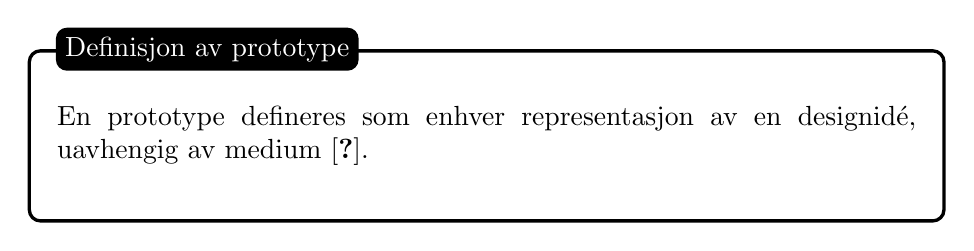
\begin{tikzpicture}
\node [mybox] (box){%
    \begin{minipage}{0.9\textwidth}
      En prototype defineres som enhver representasjon av en designidé, uavhengig av medium \cite{Houde97}.
    \end{minipage}
};
\node[fancytitle, rounded corners, right=10pt] at (box.north west) {Definisjon av prototype};
\end{tikzpicture}%


\subsection{Brukertesting}


\subsubsection{Workshop}
Tjora (2012) påpeker at valg av metode for datagenerering må reflektere hva man faktisk ønsker å finne ut, og at effektivitet bør vektlegges. “Datagenereringen må kunne frambringe mest mulig relevant og pålitelig informasjon uten unødig bruk av forskeres og deltakeres tid og ressurser”.
I tråd med \ref{chp: medvirkning} og \ref{chp:dd}, ønsket vi en brukersentrert designprosess, hvor brukerne medvirket gjennom en \emph{deltakende design workshop}.
En slik workshop åpner for at utviklere, bedriftsrepresentanter og brukere kan jobbe sammen for å avdekke utfordringer og løsninger på en svært produktiv måte. Dette vil være mest effektivt tidlig i designprosessen, da idèer ikke hemmes av eksisterende kode eller annen infrastruktur (Gaffney, 1999).

\subsubsection{Deltakere}
\subsubsection{Forberedelse}
\subsubsection{Utførelse}

\subsection{Dataanalyse}

\subsubsection{Datamaterialets kvalitet}

